% Template for PLoS
% Version 3.2 March 2016

\documentclass[10pt,letterpaper]{article}
\usepackage[top=0.85in,left=2.75in,footskip=0.75in]{geometry}

% Use adjustwidth environment to exceed column width (see example table in text)
\usepackage{changepage}

% Use Unicode characters when possible
\usepackage[utf8x]{inputenc}

% textcomp package and marvosym package for additional characters
\usepackage{textcomp,marvosym}

% fixltx2e package for \textsubscript
\usepackage{fixltx2e}

% amsmath and amssymb packages, useful for mathematical formulas and symbols
\usepackage{amsmath,amssymb}

% cite package, to clean up citations in the main text. Do not remove.
\usepackage{cite}

% Use nameref to cite supporting information files (see Supporting Information section for more info)
\usepackage{nameref,hyperref}

% line numbers
\usepackage[right]{lineno}

% ligatures disabled
\usepackage{microtype}
\DisableLigatures[f]{encoding = *, family = * }

\usepackage{booktabs}
\usepackage{xspace}
\usepackage{hyperref}
% graphicx package, useful for including eps and pdf graphics
% include graphics with the command \includegraphics
\usepackage{graphicx}


% cite package, to clean up citations in the main text. Do not remove.
\usepackage{cite}
\usepackage{subcaption}
\usepackage{rotating}

\usepackage{color} 
\usepackage{multirow}

% Remove comment for double spacing
%\usepackage{setspace} 
%\doublespacing

% Text layout
\raggedright
\setlength{\parindent}{0.5cm}
\textwidth 5.25in 
\textheight 8.75in

% Bold the 'Figure #' in the caption and separate it from the title/caption with a period
% Captions will be left justified
\usepackage[aboveskip=1pt,labelfont=bf,labelsep=period,justification=raggedright,singlelinecheck=off]{caption}
\renewcommand{\figurename}{Fig}

% Use the PLoS provided BiBTeX style
\bibliographystyle{plos2015}

% Remove brackets from numbering in List of References
\makeatletter
\renewcommand{\@biblabel}[1]{\quad#1.}
\makeatother

% Leave date blank
\date{}

% Header and Footer with logo
\usepackage{lastpage,fancyhdr,graphicx}
\usepackage{epstopdf}
\pagestyle{myheadings}
\pagestyle{fancy}
\fancyhf{}
\setlength{\headheight}{27.023pt}
\lhead{\includegraphics[width=2.0in]{PLOS-submission.eps}}
\rfoot{\thepage/\pageref{LastPage}}
\renewcommand{\footrule}{\hrule height 2pt \vspace{2mm}}
\fancyheadoffset[L]{2.25in}
\fancyfootoffset[L]{2.25in}
\lfoot{\sf PLOS}

%% Include all macros below

\newcommand{\lorem}{{\bf LOREM}}
\newcommand{\ipsum}{{\bf IPSUM}}

%% END MACROS SECTION


%% Author's settings
\def\KL{\text{KL}}





\begin{document}

\vspace*{0.2in}

% Title must be 250 characters or less.
% Please use "title case" (capitalize all terms in the title except conjunctions, prepositions, and articles).
\begin{flushleft}
{\Large
\textbf\newline{Clustering RNA-seq Expression Data using Grade of Membership Models} 
}
\newline
% Insert author names, affiliations and corresponding author email (do not include titles, positions, or degrees).
\\
Kushal K Dey \textsuperscript{1},
Chiaowen Joyce Hsiao \textsuperscript{2},
Matthew Stephens\textsuperscript{1,2}
\\
\bigskip
\textbf{1} Department of Statistics, University of Chicago, Chicago, Illinois 60637, USA
\\
\textbf{2} Department of Human Genetics, University of Chicago, Chicago, Illinois 60637, USA
\\
\bigskip


% Use the asterisk to denote corresponding authorship and provide email address in note below.
* mstephens@uchicago.edu

\end{flushleft}
% Please keep the abstract below 300 words
\section*{Abstract}
Grade of membership models, also known as ``admixture models", ``topic models" or ``Latent Dirichlet Allocation",
are a generalization of cluster models that allow each sample to have membership in multiple clusters.
These models are widely used in population genetics to model admixed individuals who have ancestry from multiple ``populations", 
and in natural language processing to model documents having words from multiple ``topics". Here we illustrate the potential for these models to cluster samples of RNA-seq gene expression data, measured on either bulk samples or single cells. 
We also provide methods to help interpret the clusters, by identifying genes that are distinctively expressed in each cluster. 
Together these methods provide an attractive summary of the primary structure in several example RNA-seq applications. Applied to
data from the GTEx project on 51 human tissues, the approach highlight similarities among biologically-related tissues and
identifies distinctively-expressed genes that largely recapitulate known biology.  Applied to single-cell expression data from 
mouse preimplantation embryos, the approach highlights both discrete and continuous variation through early embryonic development stages,
and highlights genes involved in a variety of relevant processes -- from germ cell development, through compaction and morula formation, to
the formation of inner cell mass and trophoblast at the blastocyte stage.
The methods are implemented in the BioConductor package {\tt CountClust}.


% Please keep the Author Summary between 150 and 200 words
% Use first person. PLOS ONE authors please skip this step. 
% Author Summary not valid for PLOS ONE submissions.   
\section*{Author Summary}
Lorem ipsum dolor sit amet, consectetur adipiscing elit. Curabitur eget porta erat. Morbi consectetur est vel gravida pretium. Suspendisse ut dui eu ante cursus gravida non sed sem. Nullam sapien tellus, commodo id velit id, eleifend volutpat quam. Phasellus mauris velit, dapibus finibus elementum vel, pulvinar non tellus. Nunc pellentesque pretium diam, quis maximus dolor faucibus id. Nunc convallis sodales ante, ut ullamcorper est egestas vitae. Nam sit amet enim ultrices, ultrices elit pulvinar, volutpat risus.

\linenumbers


\section*{Introduction}

Ever since large-scale gene expression measurements have been possible, clustering -- of both genes and samples -- 
has played a major role in their analysis \cite{Eisen1998, Golub1999, Alizadeh2000}.
For example, clustering of genes can identify genes that are working together or co-regulated, and clustering of samples is useful for quality control as well as identifying biologically-distinct subgroups. A wide range of clustering methods have therefore been employed in this context, including distance-based hierarchical clustering, $k$-means clustering, and self-organizing maps (SOMs); see for example \cite{D'haeseleer2005, Jiang2004} for reviews. 

Here we focus on cluster analysis of samples, rather than clustering of genes (although our methods do highlight sets of genes that distinguish each cluster). Traditional clustering methods for this problem attempt to partition samples into distinct groups that show ``similar" expression patterns. While partitioning samples in this way has intuitive appeal, 
it seems likely that the structure of a typical gene expression data set will be too complex to be fully captured by such a partitioning. Motivated by this, here we analyse expression data using grade of membership (GoM) models \cite{Erosheva2006}, which generalize clustering models to allow each sample to have partial membership in multiple clusters. That is, they allow that each sample has a proportion, or ``grade" of membership in each cluster. Such
models are widely used in population genetics to model admixture, where individuals can have ancestry from multiple populations \cite{Pritchard2000}, and in document clustering (\cite{Blei2003, Blei2009}) where each document can have membership in multiple topics. In these fields GoM models are often known as ``admixture models", and ``topic models" or ``Latent Dirichlet Allocation" \cite{Blei2003}.

In the context of RNA-seq expression data, the GoM model allows that each sample has some proportion of its RNA-seq reads coming from each cluster. For typical bulk RNA-seq experiments this assumption could be motivated by a simple -- and perhaps simplistic -- argument: each sample is a mixture of different cell types, and so clusters could represent cell types, and the membership of a sample in each cluster could represent the proportions of each cell type present. This is similar to the idea of ``deconvolution" methods that use cell-type-specific expression profiles of marker genes to estimate the concentration of different cell types in a mixture \cite{Lindsay2013}. And, indeed, the GoM model we use here is analogous to -- although different in detail from -- blind deconvolution approaches \cite{Schwartz2010,Repsilber2010}
 which estimate cell type proportions and cell type signatures jointly (see also \cite{Shen-Orr2010,Qiao2012} for semi-supervised approaches). However, we believe that the GoM model can be useful more generally to elucidate structure in expression data - not only as a way to deconvolve mixtures of cell types. For example, in single-cell expression data, where each sample is a single cell, treating each sample as a ``mixture of cell types" is clearly inappropriate, and yet we see value in the idea that there may be some ``continuous" variation in cell types, rather than (or perhaps in addition to) the purely discrete variation captured by cluster models. Indeed, the extent to which variation among cells can be described in terms of discrete clusters vs more continuous populations is a fundamental question that, when combined with appropriate single-cell RNA-seq data, the GoM models used here may ultimately help address. Further, even for bulk RNA-seq data, we argue that GoM models may yield interesting insights into heterogeneity among samples even if the inferred cluster memberships do not correspond precisely to proportions of specific cell types, as may often happen in practice.

Interestingly, although we have not previously seen GoM models applied to RNA-seq data, several software packages
for doing this already exist! \footnote{While preparing this work for publication we became aware of ongoing independent work by \cite{duVerle2016} applying GoM models to RNA-seq data.} This is because of a parallel between clustering samples based on RNA-seq counts, and clustering documents based on word counts, which means that many existing software packages for document clustering can be applied directly to RNA-seq data. Specifically, 
 the Latent Dirichlet Allocation model from \cite{Blei2003}, which is widely used to cluster documents based on their word counts, is based on a multinomial model that applies naturally and immediately to RNA-seq data. 
Whereas documents are characterized by counts of each possible word in a dictionary, RNA-seq samples
are characterized by counts of reads mapping to each possible gene (or other unit, such as transcript, or exon) in the genome. Here we use the R package {\tt maptpx} \cite{Taddy2012} to fit these models, and we add functionality for conveniently visualizing the results and annotating clusters by their most distinctive genes to help biological interpretation. These methods are implemented in the Bioconductor package {\tt CountClust} \cite{Dey2016}.



%%%%%%%%%%%%%%%%%%%
%% Results
%%%%%%%%%%%%%%%%%%%

\section*{Results}

In brief, our approach starts by summarizing RNA-seq data by a table of counts $C_{N \times G} = (c_{ng})$, where $c_{ng}$ is the number of reads from sample $n$ mapped to gene (or transcript) $g$ \cite{Oshlack2010}.  We fit a GoM model to this table of counts, which assumes that 
\begin{equation} \label{eqn:mult}
c_{n\cdot} \sim \text{Mult}(c_{n+}, p_{n\cdot}),
\end{equation}
where $c_{n\cdot}$ denotes the count vector for the $n$th sample, $c_{n+} := \sum_g c_{ng}$, and $p_{n\cdot}$ is a probability vector (non-negative entries summing to 1) whose $g$th element represents the relative expression of gene $g$ in sample $n$. 
The GoM model further assumes that 
\begin{equation} \label{eqn:gom}
p_{ng} = \sum_{k=1}^{K} q_{nk}\theta_{kg}    
\end{equation}
where $q_{n\cdot}$ is a probability vector whose $k$th element represents the grade of membership (or ``membership proportion") of
sample $n$ in cluster $k$, and $\theta_{k\cdot}$ is a probability vector whose $g$th element represents
the relative expression of gene $g$ in cluster $k$. The number of clusters $K$ is set by the analyst, and it can be helpful to explore multiple
values of $K$ (see Discussion).

Fitting this model (see Methods) results in estimated membership proportions $q$ for each sample, and estimated expression values $\theta$ for each cluster.
We visualize the membership proportions for each sample using a ``Structure plot" \cite{Rosenberg2002}, 
which is named for its widespread use in visualizing the
results of the {\it Structure} software \cite{Pritchard2000} in population genetics.
The Structure plot represents the estimated membership proportions of each sample 
as a stacked barchart, with bars of different colors representing  different clusters. Consequently samples that have similar membership proportions have
similar amounts of each color. See Fig~\ref{fig1} for example.

% Figure 1
\begin{figure}[!h]
% 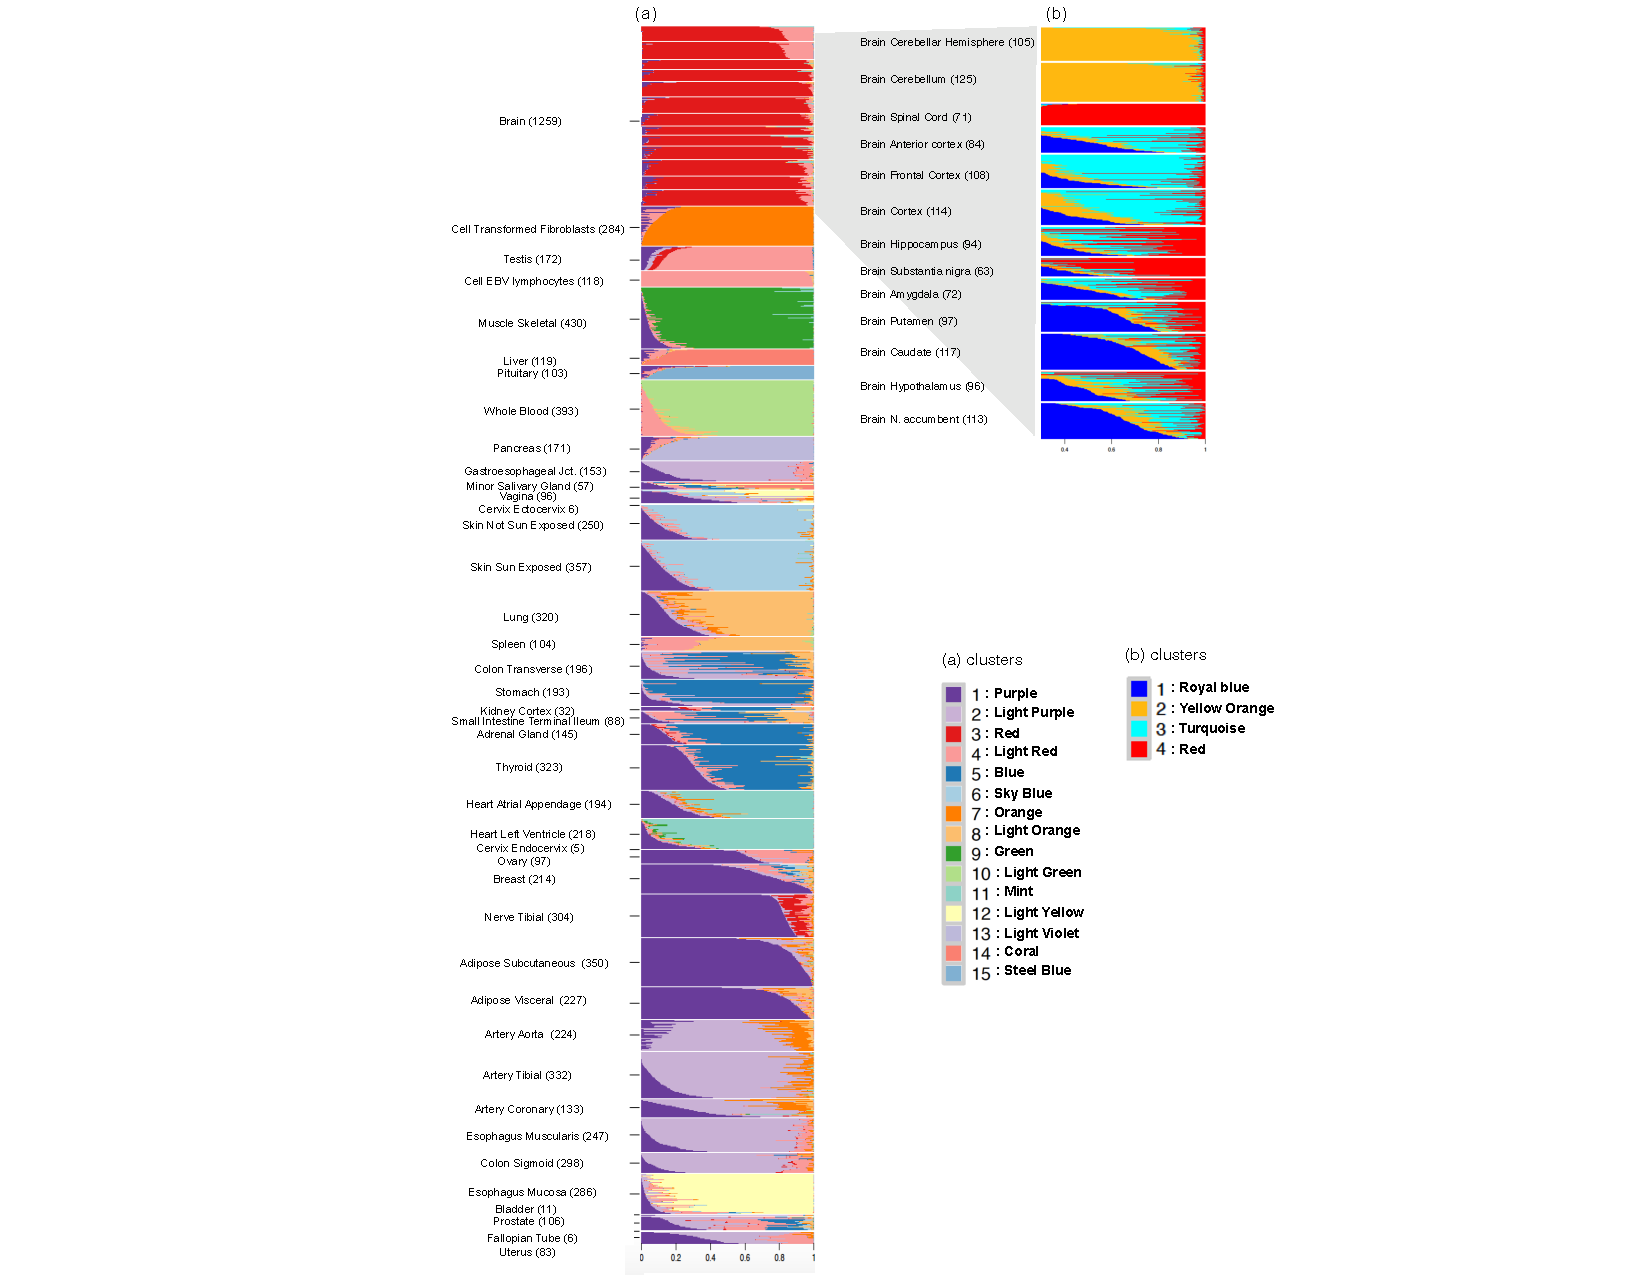
\includegraphics[height=7.5in, width=6.5in]{../plots/gtex-figures/gtex-main.pdf}
 \caption{{\bf GTEx tissue samples grades of membership.}
 (A) Structure plot of estimated membership proportions for GoM model with $K=15$ clusters fit to $8555$ tissue samples from $53$ tissues in GTEx data. Each horizontal bar shows the cluster membership proportions for a single sample, ordered so that samples from the same tissue are adjacent to one another. Within each tissue, the samples are sorted by the proportional representation of the underlying clusters. (B) Structure plot of estimated membership proportions for $K=4$ clusters fit to only the brain tissue samples. This analysis highlights finer-scale structure among the brain samples that is missed by the global analysis in (A).}
\label{fig1}
\end{figure}


\subsection*{Clustering human tissue samples using bulk RNA-seq}

We begin by illustrating the GoM model on bulk RNA expression measurements from the GTEx project (V6 dbGaP accession phs000424.v6.p1, release date: Oct 19, 2015, \url{http://www.gtexportal.org/home/}).  These data consist of per-gene read counts from RNA-seq performed on $8,555$ samples collected from $450$ human donors across $51$ tissues, lymphoblastoid cell lines, and transformed fibroblast cell-lines. We analyzed $16,069$ genes that satisfied filters (e.g.~exceeding certain minimum expression levels) that were used during eQTL analyses by the GTEx project (gene list available in \url{http://stephenslab.github.io/count-clustering/project/src/gene_annotation_2.html}). 

We applied the GoM model to these data, with $K=10,12,15$. Many of the primary patterns were consistent across these $K$, and so for brevity we focus on results for $K=15$, shown as a Structure plot in Fig~\ref{fig1}(A) (see also an alternative visualization using a 2-dimensional projection with t-SNE \cite{Maaten2008}, \cite{Maaten2014}, in Supplemental Fig \url{http://stephenslab.github.io/count-clustering/project/src/tissues_tSNE_2.html}). Reassuringly, much of the structure highlighted by these results follows the known division of samples into tissues: that is, samples from the same tissue tend to have similar membership proportions across clusters. Some tissues are represented by essentially a single cluster (e.g.~Pancreas, Whole Blood), whereas other tissues are represented as a mixture of multiple clusters (e.g.~Thyroid). Furthermore, the results highlight biological similarity among some tissues by assigning similar membership proportions to samples from those tissues.  For example, samples from different parts of the brain have similar memberships, as do the arteries (aorta, tibial and coronary) and skin (sun-exposed and un-exposed). 
 Samples from the tibial nerve have small but consistent amounts of membership in common with brain tissues, as well as larger amounts in common with the adipose tissues. Indeed, many tissues show membership this ``Adipose" cluster (cluster 1, purple in Figure), possibly reflecting, at least in some cases, contamination with adipose cells.

To help biologically interpret results we implemented methods to identify the genes and genetic processes that characterize each cluster (see Methods). Table~\ref{tab1} summarizes results for the GTEx results in Fig~\ref{fig:fig1}(A) (see also \namref{S1_Table}). 

Reassuringly, many results align with known biology. For example,  the light red cluster (cluster 4), which distinguishes Testis from other tissues, is enriched for
genes responsible for sexual reproduction and spermatogenesis etc, (e.g.: \textit{PRM2}, \textit{PRM1}, \textit{PHF7}). Similarly the light green cluster (cluster 10), which primarily distinguishes Whole Blood from other tissues, is enriched with genes responsible for immune responses (e.g. \textit{CSF3R}, \textit{IFITM2}) and hemoglobin complex and oxygen transport (e.g. \textit{HBB}, \textit{HBA1}, \textit{HBA2}). Further, digestion-related and proteolysis-related genes characterize the Pancreas cluster (cluster 13, light violet), Keratin-related genes characterize the skin cluster (cluster 6, sky blue), Myosin-related genes characterize the muscle skeletal cluster (cluster 9, green), etc. In cases where a cluster occurs in multiple tissues these biological annotations may be particularly helpful for understanding what is driving this co-membership. For example, the top four genes in the  light orange cluster (cluster 8), which is common to Lung, Spleen and Small Intestine - Terminal Ileum,  all code for surfactant proteins (specifically, B, A2, A1 and C).

\begin{table}[!hp]
\begin{adjustwidth}{-2.00in}{0in} % Comment out/remove adjustwidth environment if table fits in text column.
\footnotesize
\centering
\caption{\bf Cluster Annotations GTEx V6 data (with GO annotations).}} 
\renewcommand{\arraystretch}{1.7}
\begin{tabular}{|p{1.0in}|p{1.5in}|p{4.3in}|} 
\hline
Cluster & Top 5 Driving \qquad Genes  &  Top significant GO terms \\
\hline
1. Royal purple & \textit{NEAT1, IGFBP5, CCLN2, SRSF5, PNISR} & GO:0005654 (nucleoplasm), GO:0044428 (nuclear part), GO:0044822 (poly-A RNA binding), GO:0043233 (organelle lumen)  \\ \hline
2. Light purple & \textit{SNAP25, FBXL16, NCDN, SNCB, SLC17A7} & GO:0097458 (neuron part), GO:0007268 (synaptic transmission), GO:0030182 (neuron differentiation), GO:0022008 (neurogenesis), GO:0007267 (cell-cell signaling) \\ \hline
3. Red & \textit{FABP4, PLIN1, FASN, GPX3, LIPE} & GO:0044255 (cellular lipid metabolism), GO:0006629 (lipid metabolism), GO:0006639 (acylglycerol metabolism), GO:0045765 (angiogenesis regulation), GO:0019915 (lipid storage) \\ \hline
4. Salmon & \textit{ACTG2, MYH11, SYNM, MYLK, CSRP1} & GO:0043292 (contractile fiber), GO:0006936 (muscle contraction), GO:0015629 (actin cytoskeleton), GO:0030016 (myofibril), GO:0005925 (focal adhesion) \\ \hline
5. Denim & \textit{RGS5, MGP,  AEBP1, IGFBP7, MFGE8} & GO:0005578 (proteinaceous extracellular matrix), GO:0030198 (extracellular matrix), GO:0007155 (cell adhesion), GO:0001568 (blood vessel development) \\ \hline
6. Light denim & \textit{KRT10, KRT1, KRT2, LOR, KRT14} & GO:0008544 (epidermis development), GO:0043588 (skin development), GO:0042303 (molting cycle), GO:0042633 (hair cycle), GO:0048513 (organ development \\ \hline
7. Orange & \textit{NEB, MYH1, MYH2, MYBPC1, ACTA1} & GO:0043292 (contractile fiber), GO:0030016 (myofibril), GO:0030017 (sarcomere), GO:0003012 (muscle system process), GO:0015629 (actin cytoskeleton) \\ \hline
8. Light orange & \textit{FN1, COL1A1, COL1A2, COL3A1, COL6A3} & GO:0030198 (extracellular matrix), GO:0043062 (extracellular structure), GO:0032963 (collagen metabolism), GO:0030199 (collagen fibril organization), GO:0030574 (collagen catabolism) \\ \hline
9. Green & \textit{MBP, GFAP, MTURN, HIPK2, CARNS1} & GO:0043209 (myelin sheath), GO:0007399 (nervous system development), GO:0008366 (axon ensheathment), GO:0044430 (cytoskeletal part), GO:0005874 (microtubule) \\ \hline
10. Light green & \textit{CYP17A1, CYP11B1, PIGR, GKN1, STAR} & GO:0006694 (steroid biosynthesis), GO:0008202 (steroid metabolism), GO:0016125 (sterol metabolism), GO:0042446 (hormone biosynthesis), GO:0008207 (C21-steroid hormone metabolism) \\ \hline
%\end{tabular}
%\label{tab:tab1}
%\end{adjustwidth}
% \end{table}	
%  
%  
% 
%\begin{table}[!hp]
%%%\caption{Cluster Annotations GTEx V6 data (with GO annotations).}
%\begin{adjustwidth}{-2.00in}{0in} % Comment out/remove adjustwidth environment if table fits in text column.
%\footnotesize
%\centering
%%\caption{\bf Cluster Annotations GTEx V6 data (with GO annotations).}} \label{tab:tab1}
%\renewcommand{\arraystretch}{2}
%\begin{tabular}{|p{1.0in}|p{1.5in}|p{4.3in}|} 
%\hline
%Cluster & Top 5 Driving \qquad Genes &  Top significant GO terms \\
%\hline
11. Turquoise & \textit{MPZ, APOD, PMP22, PRX, NGFR} & GO:0008366 (axon ensheathment), GO:0048856 (anatomical structure development), GO:0007272 (ensheathment of neurons), GO:0042552 (myelination), GO:0005578 (proteinaceous extracellular matrix) \\ \hline
12. Yellow & \textit{IGHM, IGHG1, IGHG2, IGHG4, CD74} & GO:0006955 (immune response), GO:0002252 (immune effector process), GO:0003823 (antigen binding), GO:0019724 (B-cell mediated immunity), GO:0002684 (positive regulation immune system) \\ \hline
13. Sky blue & \textit{TG, PRL, GH1, PRM2, PRM1} & GO:0019953 (sexual reproduction), GO:0048232 (male gamete generation), GO:0035686 (sperm fibrous sheath), GO:0005179 (hormone activity), GO:0042403 (thyroid hormone metabolism) \\ \hline
14. Light pink & \textit{NPPA, MYH6, TNNT2, ACTC1, MYBPC3} & GO:0045333 (cellular respiration), GO:0022904 (respiratory electron transport), GO:0031966 (mitochondrial membrane), GO:0015980 (energy derivation by oxidation of organic compounds) \\ \hline
15. Light gray & \textit{KRT13, KRT4, MUC7, CRNN, KRT6A} & GO:0043230 (extracellular organelle), GO:0070062 (extracellular exosome), GO:0031982 (vesicle), GO:0008544 (epidermis development), GO:0043588 (skin development) \\ \hline
16. Gray & \textit{SFTPB�, SFTPA1, SFTPA2, SFTPC, A2M} & GO:0001525 (angiogenesis), GO:0048514 (blood vessel morphogenesis), GO:2000145 (cell motility regulation), GO:0071944 (cell periphery), GO:0009611 (response to wounding) \\ \hline
17. Brown & \textit{CSF3R, MMP25, IL1R2, SELL, VNN2} & GO:0006955 (immune response), GO:0006952 (defense response), GO:0071944 (cell periphery), GO:0005886 (plasma membrane), GO:0050776 (regulation of immune response) \\ \hline
18. Purple & \textit{PRSS1, CPA1, PNLIP, CELA3A, GP2} & GO:0007586 (digestion), GO:0004252 (serine-type endopeptidase activity), GO:0006508 (proteolysis), GO:0044241 (lipid digestion), GO:0016787 (hydrolase activity) \\ \hline 
19. Pink & \textit{HBB, HBA2, HBA1, FKBP8, HBD} & GO:0005833 (hemoglobin complex), GO:0015669 (gas transport), GO:0020037 (heme binding), GO:0031720 (haptoglobin binding), GO:0006950 (response to stress) \\ \hline 
20. Dark gray}  & \textit{ALB, HP, FGB, FGA, ORM1} & GO:0034364 (high density lipoprotein), GO:0019752 (carboxylic acid metabolism), GO:0044710 (single organism metabolism), GO:0002526 (acute inflammatory response), GO:0031982 (vesicle) \\ \hline 
\end{tabular} \label{tab:tab1}
\end{adjustwidth}
\end{table} 


Although global analysis of all tissues is useful for highlighting major structure in the data, it may miss finer-scale structure within tissues or among similar tissues. For example, here the global analysis allocated similar cluster memberships to all brain tissues,  and we suspected that these tissues may exhibit substructure that could be uncovered by analyzing the brain samples separately.  Fig~\ref{fig1}(B) shows the Structure plot for $K=4$ on only the Brain samples. The results highlight much finer-scale structure compared with the global analysis. Brain Cerebellum and Cerebellar hemisphere are essentially assigned to a separate cluster, which is enriched with genes related to cell periphery and communication (e.g. \textit{PKD1}, \textit{CBLN3})as well genes expressed largely in neuronal cells and playing a role in neuron differentiation (e.g. \textit{CHGB}). The spinal cord samples also show consistently strong membership in a single cluster, the top defining gene for the cluster being \textit{MBP} which is involved in myelination of nerves in the nervous system\cite{Hu2016}.  The other driving gene \textit{GFAP} takes part in system development by acting as a marker to distinguish astrocytes during development \cite{Baba1997}. 

The remaining samples all show membership in multiple clusters, with cortex samples being distinguished from other samples by stronger membership in a cluster (cluster 3, turquoise in Fig~\ref{fig1}(B) whose distinctive genes include \textit{ENC1}, which  interacts with actin and contributes to the organisation of the cytoskeleton during the specification of neural fate \cite{Hernandez1997}.



\subsection*{Quantitative comparison with hierarchical clustering}

We hypothesized that the model-based GoM approach might be more accurate in detecting substructure than distance-based methods, and we used the GTEx data to test this hypothesis. Specifically, for each pair of tissues in the GTEx data we assessed whether or not each clustering method correctly partitioned samples into the two tissue groups (see Methods). The GoM model was substantially more accurate in this test, succeeding in $86 \%$ of comparisons, compared with $39 \%$ for the distance-based method; Fig~\ref{fig2}. This presumably reflects the general tendency for model-based
approaches to be more efficient that distance-based approaches, provided that the model is sufficiently accurate.

% Figure 2
\begin{figure}[!h]
\caption{ {\bf Compare accuracy of GoM model versus hierarchical clustering.} For each pair of tissues from the GTEX data we assessed whether or not each method (with $K=2$ clusters) separated the samples precisely according to their actual tissue of origin, with successful separation indicated by a filled square. Some pairs of tissues (e.g. pairs of brain tissues) are more difficult to distinguish than others. Overall the GoM model is successful in $86 \%$ comparisons and the hierarchical clustering in $39 \%$ comparisons.}
\label{fig2}
\end{figure}


\subsection*{Clustering of single-cell RNA-seq data}

Recently RNA-sequencing has become viable for single cells \cite{Tang2009}, and this technology has the promise to revolutionize understanding of intra-cellular variation in expression, and regulation more generally \cite{Trapnell2015}. Although it is traditional to describe and categorize cells in terms of distinct cell-types, the actual architecture of cell heterogeneity may be more complex, and in some cases perhaps better captured by the more ``continuous"  GoM model. In this section we illustrate the potential for the GoM model to be applied to single cell data.

To be applicable to single-cell RNA-seq data, methods must be able to deal with lower sequencing depth than in bulk RNA experiments: single-cell RNA-seq data typically involve substantially lower effective sequencing depth compared with bulk experiments, due to the relatively small number of molecules available to sequence in a single cell. Therefore, as a first step towards demonstrating its potential for single cell analysis, we checked robustness of the GoM model to sequencing depth. Specifically, we repeated the analyses above after thinning the GTEx data by a factor of $10,000$ to mimic the lower sequencing depth of a typical single cell experiment.
 
For the thinned GTEx data the Structure plot for $K=15$ preserves most of the major features of the original analysis on unthinned data (\namref{S2_Fig}). For the accuracy comparisons with distance-based methods, both methods suffer reduced accuracy in thinned data, but the GoM model remains superior. For example, when thinning by a factor of $1,000$, the success rate in separating pairs of tissues is $0.32$ for the GoM model vs $0.10$ for hierarchical clustering.

Having established its robustness to sequencing depth, we now illustrate the GoM model on two single cell RNA-seq datasets, from Jaitin \textit{et al} \cite{Jaitin2014} and Deng \textit{et al} \cite{Deng2014}.  

\subsubsection*{Jaitin \text{et al}, 2014}

Jaitin \textit{et al} sequenced over $4,000$ single cells from mouse spleen. Here we analyze $1,041$ of these cells that were categorized as $CD11c+$ in the \textit{sorting markers} column of their data (\url{http://compgenomics.weizmann.ac.il/tanay/?page_id=519}), and which had total number of reads mapping to non-ERCC genes greater than $600$. We believe these cells correspond roughly to the $1,040$ cells in their Figure S7.   Our hope was that applying our method to these data would identify, and perhaps refine, the cluster structure evident in  \cite{Jaitin2014} (their Fig 2(A)-(B)). However, our method yielded rather different results (Fig~\ref{fig3}), where most cells were assigned to have membership
in several clusters. Further, the cluster membership vectors showed systematic differences among amplification batches (which in these data is also strongly correlated with sequencing batch). For example, cells in batch 1 are characterized by strong membership in the orange cluster (cluster 5) while those in batch 4 are characterized
by strong membership in both the blue and yellow clusters (2 and 6). Some adjacent batches show similar patterns - for example batches 28 and 29 have a similar visual ``palette", as do batches 32-45. And, more generally, these later batches are collectively more similar to one another than they are to the earlier batches (0-4).

% Figure 3
\begin{figure}[h!]
%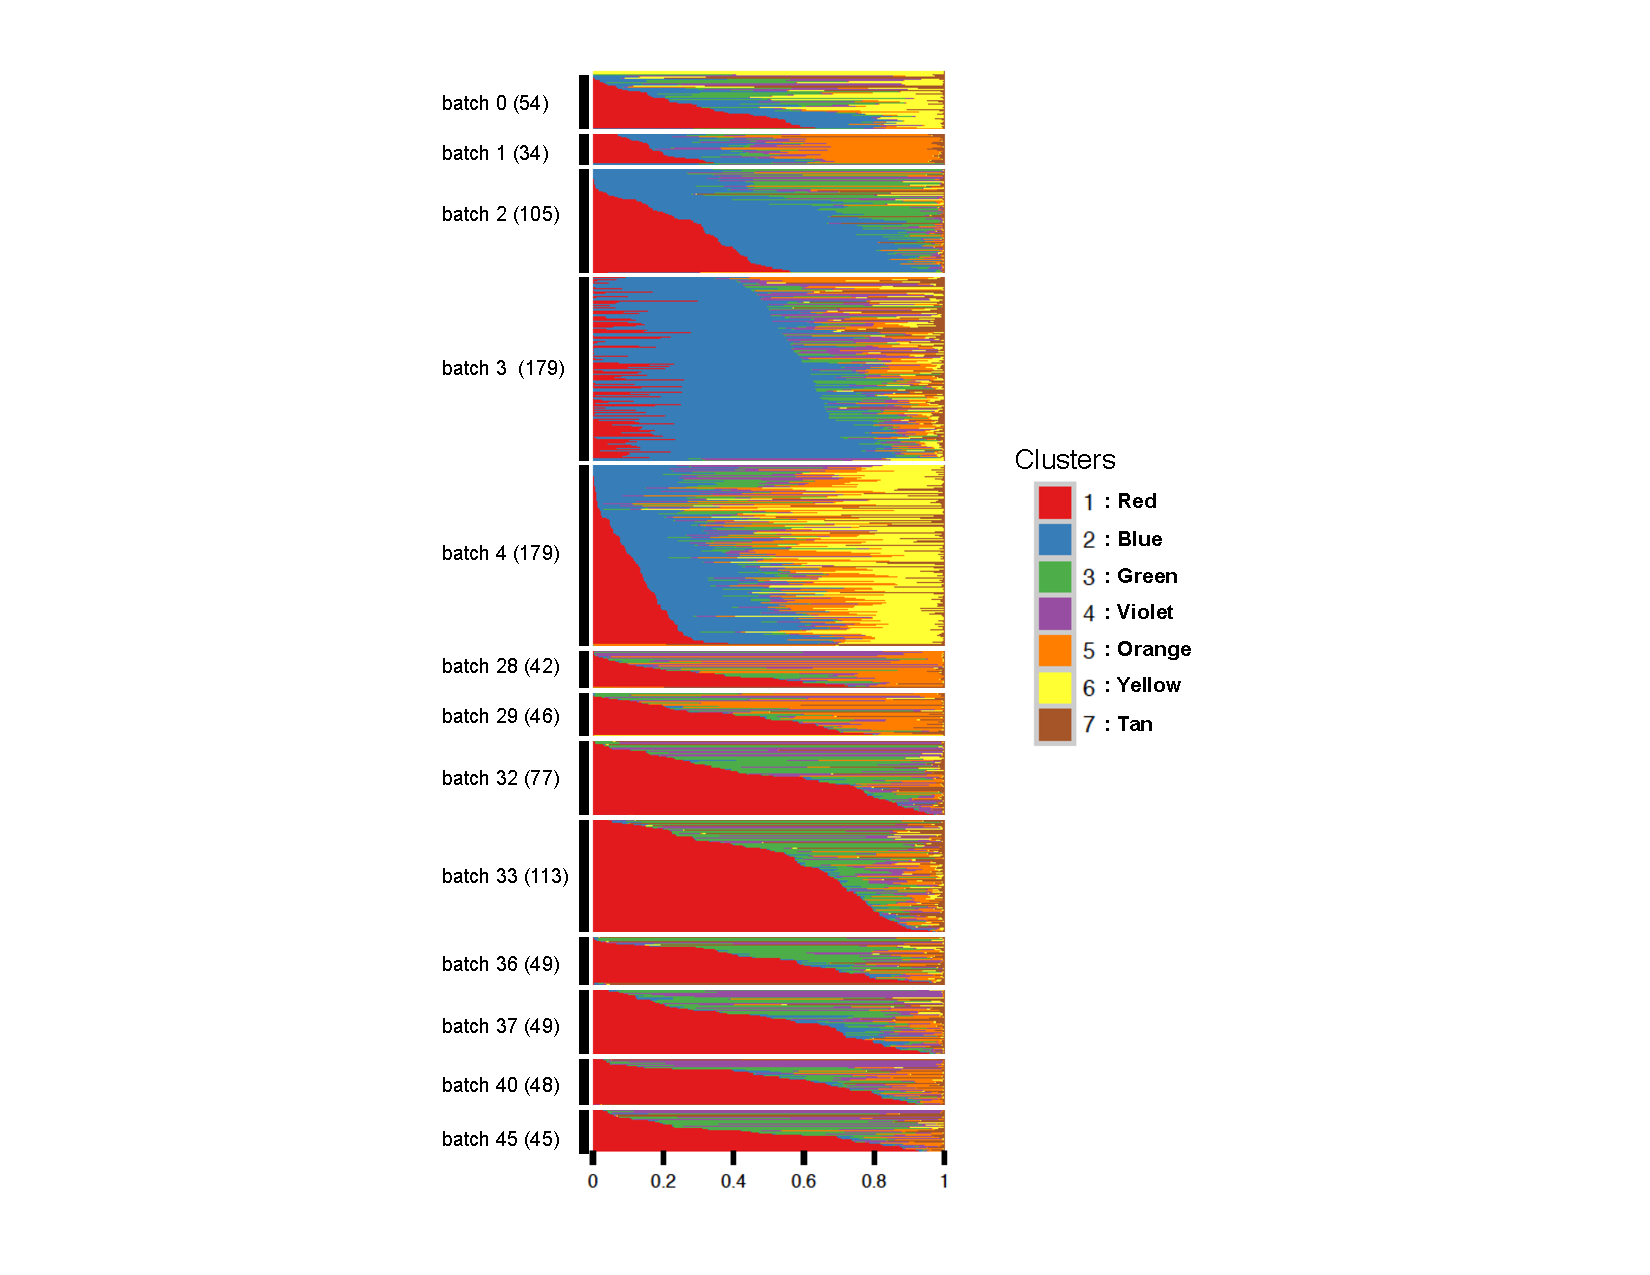
\includegraphics[height=4in, width=5.5in]{../plots/jaitin-figures/jaitin-main.pdf}
\caption{ {\bf Jaitin \textit{et al} single-cell sample estimated membership proportions.} Structure plot of estimated membership proportions for GoM model with $K=7$ clusters fit to $1,041$ single cells from \cite{Jaitin2014}. The samples (cells) are ordered so that samples from the same amplification batch are adjacent and within each batch, the samples are sorted by the proportional representation of the underlying clusters. In this analysis the samples do not appear to form clearly-defined clusters, with each sample being allocated membership in several ``clusters". Membership proportions are correlated with batch, and some groups of batches (e.g. 28-29; 32-45) show similar palettes.  These results suggest that batch effects are likely influencing the inferred structure in these data.}
\label{fig3}
\end{figure}

The fact that batch effects are detectable in these data is not particularly surprising: there is a growing recognition of the importance of batch effects in high-throughput data generally \cite{Leek2010} and in single cell data specifically \cite{Hicks2015}. And indeed, both clustering methods and the GoM model can be viewed
as dimension reduction methods, and such methods can be helpful in controlling for batch effects \cite{Leek2007, Stegle2012}. However, why these batch effects are not evident in Fig 2(A)-(B) of \cite{Jaitin2014} is unclear. 


\subsubsection*{Deng \text{et al}, 2014}

Deng \textit{et al} collected single-cell expression data of mouse preimplantation embryos from the zygote to blastocyst stage \cite{Deng2014},
with cells from four different embryos sequenced at each stage. The original analysis \cite{Deng2014} focusses on trends of allele-specific expression in early embryo development. Here we use the GoM model to assess the primary structure in these data without regard to allele-specific effects 
(i.e.~combining counts of the two alleles). Visual inspection of the Principal Components Analysis in \cite{Deng2014} suggested perhaps 6-7 clusters, 
and we focus here on results with $K=6$. 

The results from the GoM model (Fig~\ref{fig4})  clearly highlight changes in expression profiles that occur through early embryonic development stages, and enrichment analysis of the driving genes in each cluster (Table~\ref{tab3}) indicate that many of these expression changes reflect important
biological processes during embryonic preimplantation development. 

% Figure 4
\begin{figure}[h!]
%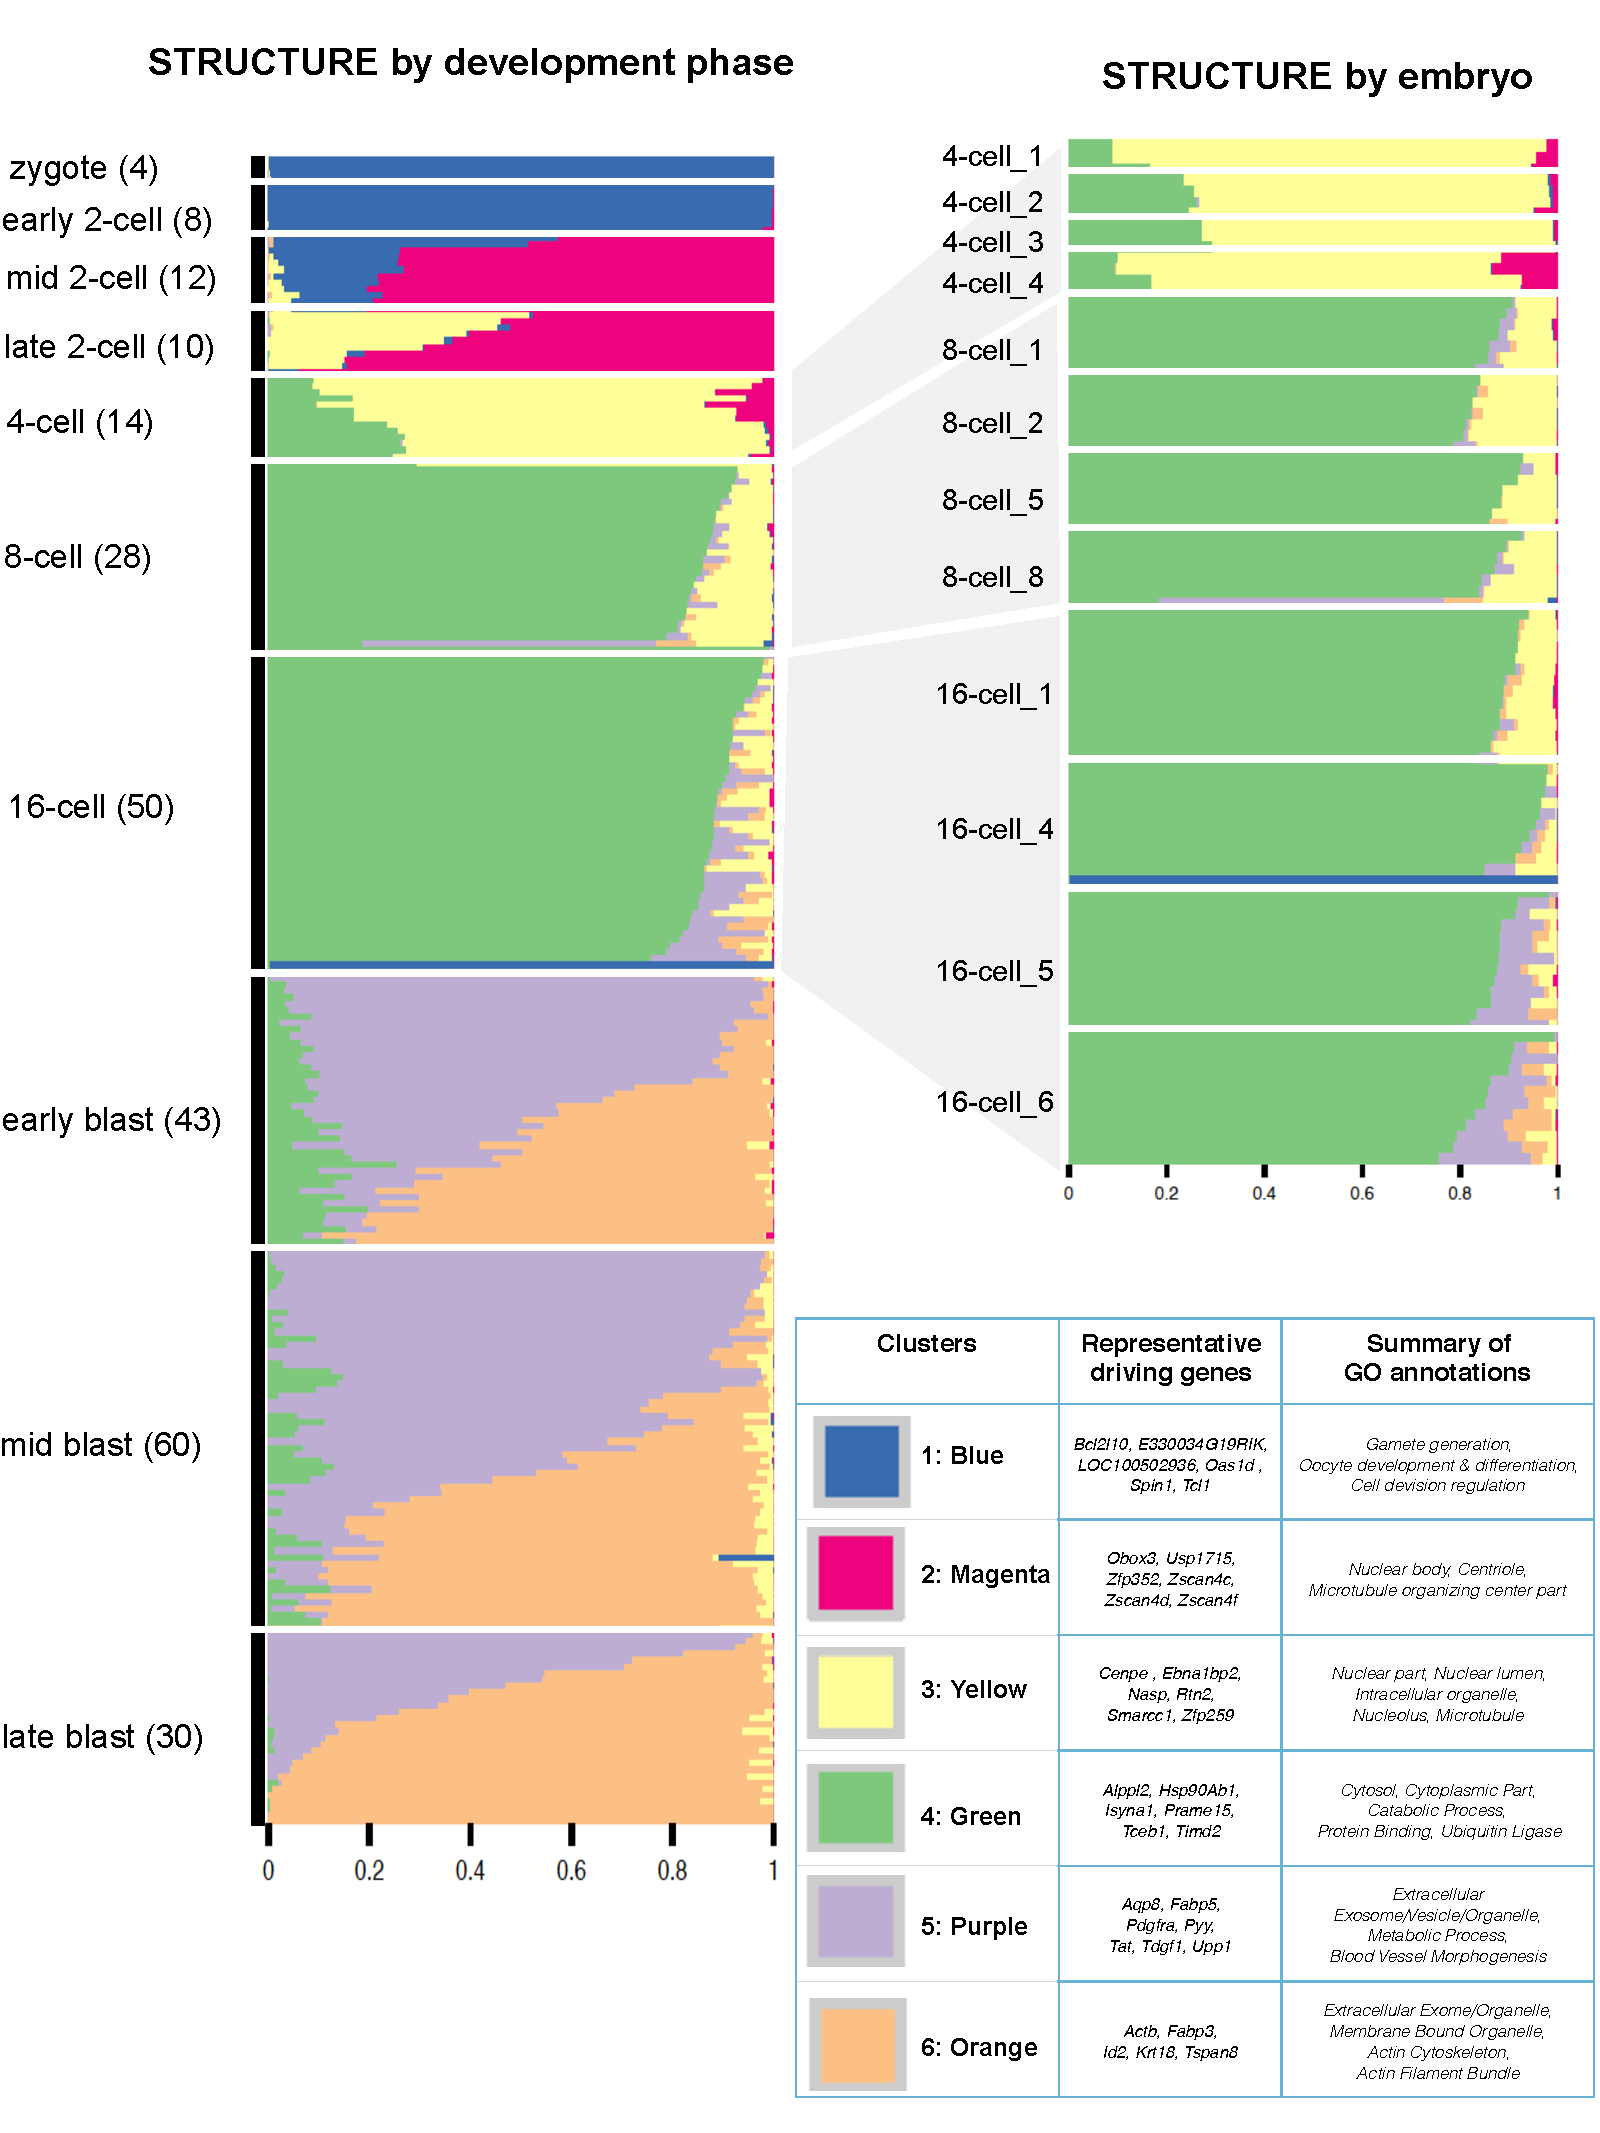
\includegraphics[height=6.5in, width=4.5in]{../plots/deng-figures/deng-main-v4.pdf}
\caption{{\bf Deng \textit{et al} single-cell sample estimated membership proportions.} Structure plot of estimated membership proportions for GoM model with $K=6$ clusters fit to $259$ single cells from  \cite{Deng2014}. The cells are ordered
by their preimplantation development phase (and within each phase, sorted by the proportional representation of the clusters). While the very earliest developmental phases 
(zygote and early 2-cell) are essentially assigned to a single cluster, others have membership in multiple clusters. Each cluster is annotated by
the genes that are most distinctively expressed in that cluster, and by the gene ontology categories for which these distinctive genes are most enriched (see Table \ref{tab3} for more extensive annotation results). See text for discussion of biological processes driving these results.}
\label{fig4}
\end{figure}


In more detail: Initially, at the zygote and early 2-cell stages, the embryos are represented by a single cluster (blue in Fig~ \ref{fig4}) that
 is enriched with genes responsible for germ cell development (e.g., \textit{Bcl2l10} \cite{Yoon2009}, \textit{Spin1} \cite{Evsikov2009}). Moving through subsequent stages the grades of membership evolve to a mixture of blue and magenta clusters (mid 2-cell), a mixture of magenta and yellow clusters (late 2-cell) and a mixture of yellow and green (4-cell stage). The green cluster then becomes more prominent in the 8-cell and 16-cell stages, before dropping  substantially in the early and mid-blastocyst stages. That is, we see a progression in the importance of different clusters
through these stages, from the blue cluster, moving through magenta and yellow to green. By examining the genes distinguishing each cluster we see that this progression reflects the changing relative importance of several fundamental biological processes. The magenta cluster is driven by genes responsible for the beginning of transcription of zygotic genes (e.g., \textit{Zscan4c-f} \cite{Falco2007}), which takes place in the late 2-cell stage of early mouse embryonic development. The yellow cluster is enriched for genes responsible for heterochromation \textit{Smarcc1} \cite{Schaniel2009} and chromosome stability \textit{Cenpe} \cite{{Putkey2002}}. And the green cluster is enriched for cytoskeletal genes (e.g., \textit{Fbxo15}) and cytoplasm genes (e.g., \textit{Tceb1}, \textit{Hsp90ab1}), all of which are essential for compaction at the 8-cell stage and morula formation at the 16-cell stage. 

Finally, during the blastocyst stages two new clusters (purple and orange in Fig~\ref{fig4}) dominate.
The orange cluster is enriched with genes involved in the formation of outer trophoblast cells (e.g., \textit{Tspan8}, \textit{Krt8}, \textit{Id2} \cite{Guo2010}), while the purple cluster is enriched with genes responsible for the formation of inner cell mass (e.g., \textit{Pdgfra}, \textit{Pyy} \cite{Hou2007}). 
Thus these two clusters are consistent with the two cell lineages, the trophectoderm
and the primitive endoderm, that make up the majority of
the cells of the blastocyst \cite{Rossant1995}. Interestingly, however, the cells do not appear to fall into two distinct and clearly-separated populations
-- at least, not in terms of their expression patterns -- but rather show a continuous
range of memberships in these two clusters, even in the late blastocyst stage.

In addition to these trends across development stages, the GoM results also highlight some embryo-level effects in the early stages (Fig~\ref{fig4}). Specifically, cells from the same embryo sometimes show greater similarity than cells from different embryos. For example, while all cells from the 16-cell stage have high memberships in the green cluster, cells from two of the embryos at this stage have memberships in both the purple and yellow clusters, while the other two embryos have memberships only in the yellow cluster. 

Finally, we note that, like clustering methods, the GoM model can be helpful in exploratory data analysis and quality control. Indeed, the GoM results highlight a few single cells as outliers. For example, a cell from a 16-cell embryo is represented by the blue cluster - a cluster that represents cells at the zygote and early 2-cell stage. Also, a cell from an 8-stage embryo has strong membership in the purple cluster - a cluster that represents cells from the blastocyst stage. 
It would seem prudent to consider excluding these cells from subsequent analyses of these data.


%%%%%%%%%%%%%%%%%%%%%%%%%
%% <--- Discussion
%%%%%%%%%%%%%%%%%%%%%%%%%

\section*{Discussion}

Our goal here is to highlight the potential for GoM models to elucidate structure in RNA-seq data from both single cell sequencing and bulk sequencing of pooled cells. We also provide tools to identify which genes are most distinctively expressed in each cluster, to aid interpretation of results. As our applications illustrate, these methods have the potential to highlight biological processes underlying the cluster structure identified.

The GoM model has several advantages over distance-based hierarchical methods of clustering. At the most basic level model-based methods are often more accurate than distance-based methods. Indeed, in our simple test on the GTEx data the model-based GoM approach more accurately separated samples into ``known" clusters. However, there are also other subtler benefits of the GoM model. Because the GoM model does not assume a strict ``discrete cluster" structure, but 
rather allows that each sample has a proportion of membership in each cluster, it can provide insights into how well a 
particular dataset really fits a ``discrete cluster" model. For example, consider our results for the data from Jaitin \textit{et al} \cite{Jaitin2014} and Deng \textit{et al} \cite{Deng2014}: in both cases most samples are assigned to multiple clusters, although the results are closer to ``discrete" for the latter than the former.
The GoM model is also better able to represent the situation where there is not really a single clustering of the samples,
but where samples may cluster differently at different genes. For example, in the GTEx data, the lung samples share memberships in common with both the spleen and adipose-related tissues. This pattern is clearly visible in the Structure plot (Fig~\ref{fig1}) but would be hard to discern from a standard hierarchical clustering. 

GoM models also have close connections with dimension reduction techniques such as factor analysis, principal components analysis and non-negative matrix factorization. All of these methods can also be used for RNA-seq data, and may often be useful. See  \cite{Engelhardt2010} for discussion of 
relationships among these methods in the context of inferring population genetic structure. While not arguing that the GoM model is uniformly superior to these other methods, we believe our examples illustrate the appeals of the approach. In particular, we would argue that for the GTEx data, the Structure plot (Fig~\ref{fig1}) combined with the cluster annotations (Table~\ref{tab1}) provide a more visually and biologically appealing summary of the data than would a principal components analysis.

Fitting GoM models can be computationally-intensive for large data sets. For the datasets we considered here the computation time ranged from $12$ minutes for the data from \cite{Deng2014} ($n=259; K=6$), through $33$ minutes for the  data from \cite{Jaitin2014} ($n=1,041; K=7$) to 3,297 minutes for the GTEx data ($n=8,555; K=15$).  Computation time can be reduced by fitting the model to only the most highly expressed genes, and we often use this strategy to get quick initial results for a dataset. Because these methods are widely used for clustering very large document datasets there is considerable ongoing interest in computational speed-ups for very large datasets, with ``on-line" (sequential) approaches capable of dealing with millions of documents \cite{Hoffman2010} that could be useful in the future for very large RNA-seq datasets. 

A thorny issue that arises when fitting these types of model is how to select the number of clusters, $K$. Like many software packages for fitting these models, the {\tt maptpx} package implements a measure of model fit that provides one useful guide. However, it is worth remembering that in practice there is unlikely to be a ``true" value of $K$, and results from different values of $K$ may complement one another rather than merely competing with one another. For example, seeing how the fitted model evolves as $K$ increases is one way to capture some notion of hierarchy in the clusters identified \cite{Rosenberg2002}. More generally it is often
fruitful to analyse data in multiple ways using the same tool: for example our GTEx analyses illustrate how 
analysis of subsets of the data (in this case the brain samples) can complement analyses of the entire data.

The version of the GoM model fitted here is relatively simple, and could certainly be embellished. For example,
the model allows the expression of each gene in each cluster to be a free parameter, whereas we might expect expression of most genes to be ``similar" across clusters. This is analogous to the idea in population genetics applications that allele frequencies in different populations may
be similar to one another \cite{Falush2003}, or in document clustering applications that most words may not differ appreciably in frequency in different topics.  In population genetics applications incorporating this idea into the model, by using a correlated prior distribution on these frequencies, 
can help improve identification of subtle structure \cite{Falush2003} and we would expect the same to happen here for RNA-seq data.




%%%%%%%%%%%%%%%%%%%
%% Methods
%%%%%%%%%%%%%%%%%%%

\section*{Materials and Methods}

\subsection*{Model Fitting}

We use the {\tt maptpx} R package \cite{Taddy2012} to fit the GoM model (Eq~(\ref{eqn:mult},\ref{eqn:gom})), which is also known as ``Latent Dirichlet Allocation" (LDA). The {\tt maptpx} package fits this model using an EM algorithm to perform Maximum a posteriori (MAP)  estimation of the parameters $q$ and $\theta$. See \cite{Taddy2012} for details.

\subsection*{Visualizing Results}

In addition to the Structure plot, we have also found it useful to visualize results using t-distributed Stochastic Neighbor Embedding (t-SNE), which is a method for visualizing high dimensional datasets by placing them in a two dimensional space, attempting to preserve the relative distance between nearby samples \cite{Maaten2014, Maaten2008}. Compared with the Structure plot our t-SNE plots contain less information, but can better emphasize clustering of samples that have similar membership proportions in many clusters. Specifically, t-SNE tends to place samples with similar membership proportions together in the two-dimensional plot, forming visual ``clusters" that can be identified by eye (e.g. \nameref{S1_ Fig}). This may be particularly helpful in settings where no external information is available to aid in making an informative Structure plot. 


\subsection*{Cluster annotation}

To help biologically interpret the clusters, we developed a method to identify which genes are most distinctively differentially expressed in each cluster. 
(This is analogous to identifying ``ancestry informative markers" in population genetics applications \cite{Rosenberg2005}.)
 Specifically, for each cluster $k$ we measure the distinctiveness of gene $g$ with respect to any other cluster $l$ using
\begin{equation}
\KL^{g} [k,l] : = \theta_{kg} \; log \frac{\theta_{kg}}{\theta_{lg}} + \theta_{lg} - \theta_{kg},
\end{equation}
which is the Kullback--Leibler divergence of the Poisson distribution with parameter $\theta_{kg}$ to the Poisson distribution with parameter $\theta_{lg}$. 
For each cluster $k$, we then define the distinctiveness of gene $g$ as 
\begin{equation}
D^{g}[k] = \underset{l \neq k}{\min} \; \KL^{g} [k, l].
\end{equation}
The higher $D^g[k]$, the larger the role of gene $g$ in distinguishing cluster $k$ from all other clusters. 
Thus, for each cluster $k$ we identify the genes with highest $D^{g}[k]$ as the genes driving the cluster $k$. 
We annotate the biological functions of these individual genes using the {\tt mygene} R Bioconductor package  \cite{Thompson2014}. 

For each cluster $k$, we filter out a number of genes (top $100$ for the Deng \textit{et al} data \cite{Deng2014} and GTEx V6 data \cite{GTEX2013}) with highest $D^{g}[k]$ value and perform a gene set over-representation analysis of these genes against all the other genes in the data representing the background. To do this, we used ConsensusPathDB database (\url{http://cpdb.molgen.mpg.de/})  \cite{Kamburov2013, Pentchev2010}. See Tables~\ref{tab1} - \ref{tab2} and Table~\ref{tab3} for the top significant gene ontologies driving each cluster in the GTEx V6 data and the Deng \textit{et al} data respectively. 

% Table 2
\begin{table}[!hp]
\begin{adjustwidth}{-2.00in}{0in} % Comment out/remove adjustwidth environment if table fits in text column.
\footnotesize
\centering
\caption{\bf Cluster Annotations for GTEx V6 Brain data.}} 
\renewcommand{\arraystretch}{1.7}
\begin{tabular}{|p{1.0in}|p{1.5in}|p{4.3in}|} 
 \hline
 Cluster & Top 5 Driving \qquad Genes & Top significant GO terms \\
\hline
 1. Royal blue  & \textit{ATP1A2, CLU, PPP1R1B, APOE, GLUL} & GO:0044707 (single-multicellular organism process), GO:0005615 (extracellular space), GO:0048731 (system development), GO:0007154 (cell communication), GO:0007275 (multicellular organismal development), GO:0007267 (cell-cell signaling) \\
\hline
2. Yellow orange & \textit{PKD1, CBLN3, COL27A1, CHGB, PPFIA4} & GO:0005886 (plasma membrane), GO:0071944 (cell periphery), GO:0097458 (neuron part), GO:0030182 (neuron differentiation), GO:0007154 (cell communication), GO:0098794 (postsynapse), GO:0050803 (regulation of synapse structure/activity) \\
\hline
3. Turquoise & \textit{ENC1, CALM2, MAP1A, CALM3, YWHAH} & GO:0007268 (synaptic transmission), O:0097458 (neuron part), GO:0007267 (cell-cell signalling), GO:0031175 (neuron projection development), GO:0030182 (neuron differentiation), GO:0042995 (cell projection) \\
\hline
4. Red & \textit{MBP, GFAP, TF, MTURN, PAQR6} & GO:0043209 (myelin sheath), GO:0007275 (multicellular organism development), GO:0031982 (vesicle), GO:0048731 (system development), GO:0007272 (ensheathment of neurons), GO:0008366 (axon ensheathment)\\
\hline	
\end{tabular} \label{tab:tab2}
\end{adjustwidth}
 \end{table}


% Table 3
\begin{table}[!hp]
\begin{adjustwidth}{-2.00in}{0in} % Comment out/remove adjustwidth environment if table fits in text column.
\footnotesize
\centering
\caption{\bf Cluster Annotations for Deng et al (2014) data.}} 
\renewcommand{\arraystretch}{1.7}
\begin{tabular}{|p{1.0in}|p{1.5in}|p{4.3in}|}
\hline
Cluster & Top 10 Driving \qquad Genes &  Top significant GO terms \\
\hline
1. Blue 
& \textit{Bcl2l10}, \textit{Tcl1}, {\textit{E330034G19Rik}, \textit{LOC100502936}, \textit{Oas1d}, \textit{AU022751}, \textit{Spin1}, \textit{Khdc1b}, \textit{D6Ertd527e}, \textit{Btg4}
%& \textit{Bcl2l10} (Bcl2 like 10), \textit{Tcl1} (T cell lymphoma breakpoint 1), {\textit{E330034G19Rik} (RIKEN cDNA E330034G19 gene), \textit{LOC100502936}, \textit{Oas1d} ($2^{'}$-$5^{'}$ oligoadenylate synthetase 1D), \textit{AU022751} (expressed sequence AU022751), \textit{Spin1} (spindlin 1), \textit{Khdc1b} (KH domain containing 1B, \textit{D6Ertd527e} (DNA segment, Chr 6, ERATO Doi 527, expressed), \textit{Btg4}(B cell translocation gene 4) 
& GO:0007276 (gamete generation), GO:0032504 (multicellular organism reproduction), GO:0044702 (single organism reproduction), GO:0048477 (oogenesis), GO:0048599 (oocyte development), GO:0009994 (oocyte differentiation), GO:0051321 (meiotic cell cycle), GO:0006306 (DNA methylation), GO:0051302 (regulation of cell division)\\
\hline
2. Magenta
& \textit{Obox3}, \textit{Zfp352}, \textit{Gm8300}, \textit{Usp17l5}, \textit{BB287469}, \textit{Rfpl4b}, \textit{Gm2022}, \textit{Gm5662}, \textit{Gm11544 }, \textit{Gm4850}
%& \textit{Obox3} (oocyte specific homeobox 3)
%, \textit{Zfp352} (zinc finger protein 352)
%, \textit{Gm8300} (predicted gene 8300)
%, \textit{Usp17l5}
%, \textit{BB287469} (expressed sequence BB287469)
%, \textit{Rfpl4b } (ret finger protein-like 4B)
%, \textit{Gm2022}(predicted pseudogene 2022)
%, \textit{Gm5662} (predicted gene 5662)
%, \textit{Gm11544 } (predicted gene 11544)
%, \textit{Gm4850}(THO complex 4 pseudogene) 
& GO:0016604 (nuclear body), GO:0005814 (centriole), GO:0044450 (microtubule organizing center part) \\ 			
\hline
3. Yellow
& \textit{Rtn2}, \textit{Ebna1bp2}, \textit{Zfp259}, \textit{Nasp}, \textit{Cenpe}, \textit{Rnf216}, \textit{Ctsl}, \textit{Tor1b}, \textit{Ankrd10}, \textit{Lamp2}
%& \textit{Rtn2} (reticulon 2, Z-band associated protein)
%, \textit{Ebna1bp2} (EBNA1 binding protein 2)
%, \textit{Zfp259}
%, \textit{Nasp} (nuclear autoantigenic sperm protein, histone-binding)
%, \textit{Cenpe}(centromere protein E)
%, \textit{Rnf216} (ring finger protein 216)
%, \textit{Ctsl} (cathepsin L)
%, \textit{Tor1b} (torsin family 1, member B)
%, \textit{Ankrd10}(ankyrin repeat domain 10)
%, \textit{Lamp2} (lysosomal-associated membrane protein 2)
& GO:0044428 (nuclear part), GO:0031981 (nuclear lumen), GO:0070013 (intracellular organelle lumen), GO:0005730 (nucleolus), GO:0005654 (nucleoplasm),  GO:0003723 (RNA binding), GO:0005874 (microtubule), GO:0043229 (intracellular organelle)\\
\hline
4. Green  
&  \textit{Timd2}, \textit{Isyna1}, \textit{Alppl2}, \textit{Prame15}, \textit{Hsp90ab1}, \textit{Fbxo15}, \textit{Tceb1}, \textit{Gpd1l}, \textit{Pemt}, \textit{Hsp90aa1}
%&  \textit{Timd2} (T cell immunoglobulin and mucin domain containing 2)
%, \textit{Isyna1} (myo-inositol 1-phosphate synthase A1)
%, \textit{Alppl2} (alkaline phosphatase, placental-like 2)
%, \textit{Prame15} (preferentially expressed antigen in melanoma like 5)
%, \textit{Hsp90ab1} (heat shock protein 90 alpha (cytosolic), class B member 1)
%, \textit{Fbxo15} (F-box protein 15)
%, \textit{Tceb1} (transcription elongation factor B (SIII), polypeptide 1)
%, \textit{Gpd1l } (glycerol-3-phosphate dehydrogenase 1-like)
%, \textit{Pemt} (phosphatidylethanolamine  \; N-methyltransferase)
%, \textit{Hsp90aa1} (heat shock protein 90, alpha (cytosolic), class A member 1) 
& GO:0005829 (cytosol), GO:0044444 (cytoplasmic part), GO:1901575 (organic substance catabolic process), GO:0000151 (ubiquitin ligase com- plex),  GO:0009056 (catabolic process), GO:0072655 (protein localization mitochondrion), GO:0044265 (cellular macromolecule catabolic process), GO:0051082 (unfolded protein binding), GO:0023026 (MHC class II protein complex binding), GO:0055131 (C3HC4-type RING finger domain binding) \\ 
\hline
5. Purple & \textit{Upp1}, \textit{Tdgf1}, \textit{Aqp8}, \textit{Fabp5}, \textit{Tat}, \textit{Pdgfra}, \textit{Pyy}, \textit{Prdx1}, \textit{Col4a1}, \textit{Spp1}
%, \textit{Tdgf1} (teratocarcinoma-derived growth factor 1)
%, \textit{Aqp8} (aquaporin 8)
%, \textit{Fabp5} (fatty acid binding protein 5, epidermal, protects against atherosclerosis, diet-induced obesity, insulin resistance and experimental autoimmune encephalomyelitis)
%, \textit{Tat} (tyrosine aminotransferase, regulated by glucocorticoid and polypeptide hormones)
%, \textit{Pdgfra} (platelet derived growth factor receptor, alpha polypeptide)
%, \textit{Pyy } (peptide YY)
%, \textit{Prdx1} (peroxiredoxin 1)
%, \textit{Col4a1} (collagen, type IV, alpha 1)
%, \textit{Spp1} (secreted phosphoprotein 1) 
& GO:0070062 (extracellular exosome), GO:0043230 (extracellular organelle), GO:1903561 (extracellular vesicle), GO:0006950 (response to stress), GO:0006979 (response to oxidative stress), GO:0044710 (metabolic process), GO:0048514 (blood vessel morphogenesis), GO:0001944 (vasculature development), GO:0030198 (extracellular matrix organization) \\ 
\hline
6. Orange & \textit{Actb}, \textit{Krt18}, \textit{Fabp3}, \textit{Id2}, \textit{span8}, \textit{Gm2a}, \textit{Lgals1}, \textit{Adh1}
, \textit{Lrp2}, \textit{BC051665}
%, \textit{Krt18} (keratin 18)
%, \textit{Fabp3} (fatty acid binding protein 3, muscle and heart)
%, \textit{Id2} (inhibitor of DNA binding 2)
%, \textit{span8} (tetraspanin 8)
%, \textit{Gm2a} (GM2 ganglioside activator protein)
%, \textit{Lgals1} (lectin, galactose binding, soluble 1)
%, \textit{Adh1} (alcohol dehydrogenase 1, class I)
%, \textit{Lrp2} (low density lipoprotein receptor-related protein 2)
%, \textit{BC051665} (cDNA sequence BC051665)
& GO:0065010 (extracellular membrane-bounded organelle), GO:0070062 (extracellular exosome),  GO:0043230 (extracellular organelle), GO:1903561 (extracellular vesicle), GO:0031982 (vesicle), GO:0048468 (cell development), GO:0030036 (actin cytoskeleton and organization), GO:0032432 (actin filament bundle),  GO:0005912 (adherens junction)\\ 
\hline
\end{tabular} \label{tab:tab3}
\end{adjustwidth}
 \end{table}






%\subsection*{Comparison with hierarchical clustering}
%
%We compared the GoM model with a distance-based hierarchical clustering algorithm by applying both methods to samples from pairs of tissues from the GTEx project, and assessed their accuracy in
%separating samples according to tissue.  For each pair of tissues  we randomly selected $50$ samples from the pool of all samples coming from these tissues. For the hierarchical clustering approach we cut the dendogram at $K=2$, and checked whether or not this cut partitions the samples into the two tissue groups. 
%(We applied hierarchical clustering using Euclidean distance, with both complete and average linkage; results were similar and so we showed results only for complete linkage.) 
%
%For the GoM model we analysed the data with $K=2$, and sorted the samples by their membership in cluster 1. We then partitioned the samples at the point of the steepest fall in this membership, and again we checked whether this cut partitions the samples into the two tissue groups. Fig~\ref{fig2} shows, for each pair of tissues, whether each method successfully partitioned the samples into the two tissue groups.
%
%
%\subsection*{Thinning}
%
%We used ``thinning" to simulate lower-coverage data from the original higher-coverage data.. 
%Specifically, if $c_{ng}$ is the counts of number of reads mapping to gene $g$ for sample $n$ for the original data, we simulated thinned counts $t_{ng}$ using 
%\begin{equation}
%t_{ng} \sim Bin (c_{ng}, p_{thin})
%\end{equation}
%where $p_{thin}$ is a specified thinning parameter.
%
%
%\subsection*{Code Availability}
%
%Our methods are implemented in an R BioConductor package {\tt CountClust} (\url{https://www.bioconductor.org/packages/3.3/bioc/html/CountClust.html}). The working version of the package is maintained at \url{https://github.com/kkdey/CountClust}. Code for reproducing analyses reported in this manuscript is available at \url{http://stephenslab.github.io/count-clustering/}.




%%%%%%%%%%%%%%%%%%%%%%%%%
%% <--- Supporting information
%%%%%%%%%%%%%%%%%%%%%%%%%
% Include only the SI item label in the paragraph heading. Use the \nameref{label} command to cite SI items in the text.

\section*{Supporting Information}
\paragraph*{S1 Fig.}
\label{S1_Fig}
{\bf Structure plot of the thinned GTEx V6 data with K=15.} (A) $p_{thin}=0.01$ and (B) $p_{thin}=0.0001$. The patterns in two plots closely correspond to the plot in Fig~\ref{fig1}(A), though are a bit more noisy than compared to the unthinned version.
    
\paragraph*{S2 Fig.}
\label{S2_Fig}
{\bf Compare ``accuracy" of GoM model versus hierarchical clustering on thinned GTEx data.} (A)-(B) thinning parameter $p_{thin}=0.01$, and (C)-(D) $p_{thin}=0.0001$. For each pair of tissues from the GTEx data we assessed whether or not each clustering method (with $K=2$ clusters) separated the samples according to their actual tissue of origin, with successful separation indicated by a filled square. Thinning deteriorates accuracy compared with the unthinned data (Fig~\ref{fig2}), but even then the model-based method remains more successful than the hierarchical clustering in separating the samples by tissue or origin.

\paragraph*{S1 Table.}
\label{S1_Table}
{\bf Cluster Annotations GTEx V6 data of all tissue samples with top gene summaries.} 

\paragraph*{S2 Table.}
\label{S2_Table}
{\bf Cluster Annotations GTEx V6 Brain data with top gene summaries.} 

\paragraph*{S3 Table.}
{\bf Deng et al (2014) cluster top GO annotations.} )
(A) Blue cluster (Cluster 1) \label{S3_Table(A)}, 
(B) Magneta cluster (Cluster 2) \label{S3_Table(B)}, 
(C) Yellow cluster (Cluster 3) \label{S3_Table(C)}, 
(D) Green cluster (Cluster 4) \label{S3_Table(D)}, 
(E) Purple cluster (Cluster 5) \label{S3_Table(E)}, 
(F) Orange cluster (Cluster 6) \label{S3_Table(F)}.


%%%%%%%%%%%%%%%%%%%%%%%%
% <--- Acknowledgements
%%%%%%%%%%%%%%%%%%%%%%%%

\section*{Acknowledgments}
The Genotype-Tissue Expression (GTEx) Project was supported by the Common Fund of the Office of the Director of the National Institutes of Health. Additional funds were provided by the NCI, NHGRI, NHLBI, NIDA, NIMH, and NINDS. Donors were enrolled at Biospecimen Source Sites funded by NCI $\ $ SAIC-Frederick, Inc. (SAIC-F) subcontracts to the National Disease Research Interchange (10XS170), Roswell Park Cancer Institute (10XS171), and Science Care, Inc. (X10S172). The Laboratory, Data Analysis, and Coordinating Center (LDACC) was funded through a contract (HHSN268201000029C) to The Broad Institute, Inc. Biorepository operations were funded through an SAIC-F subcontract to Van Andel Institute (10ST1035). Additional data repository and project management were provided by SAIC-F (HHSN261200800001E). The Brain Bank was supported by a supplements to University of Miami grants DA006227 $\&$ DA033684 and to contract N01MH000028. Statistical Methods development grants were made to the University of Geneva (MH090941 $\&$ MH101814), the University of Chicago (MH090951, MH090937, MH101820, MH101825), the University of North Carolina - Chapel Hill (MH090936 $\&$ MH101819), Harvard University (MH090948), Stanford University (MH101782), Washington University St Louis (MH101810), and the University of Pennsylvania (MH101822). The data used for the analyses described in this manuscript were obtained from: the GTEx Portal on 10/19/2015 and  dbGaP accession number phs000424.v6.p1.

We thank Matt Taddy, Amos Tanay and Effi Kenigsberg for helpful discussions. We thank Po-Yuan Tung and John Blischak for helpful comments on a draft manuscript.

\nolinenumbers

\section*{Disclosure Declaration}

The authors have no conflict of interest. 

\nolinenumbers



%%%%%%%%%%%%%%%%%%%%%%%%
% <--- References
%%%%%%%%%%%%%%%%%%%%%%%%

\begin{thebibliography}{10}

%\bibitem{Sanders2014} 
%S Anders, T P Pyl, W Huber.
%\textit{HTSeq :  A Python framework to work with high-throughput sequencing data}. 
%Bioinformatics, 2014, in print; online at doi:10.1093/bioinformatics/btu638
%
%\bibitem{Li2009} 
%Li H.*, Handsaker B.*, Wysoker A., Fennell T., Ruan J., Homer N., Marth G., Abecasis G., Durbin R. and 1000 Genome Project Data Processing Subgroup.
%\textit{The Sequence alignment/map (SAM) format and SAMtools}. 
%Bioinformatics, 2009, 25, 2078-9. [PMID: 19505943]
%
%\bibitem{Liao2013}
%Liao Y, Smyth GK and Shi W. 
%\textit{The Subread aligner: fast, accurate and scalable read mapping by seed-and-vote}.
%Nucleic Acids Research, 2013, 41, pp. e108.

%\bibitem{Robinson2010}
%Robinson MD, McCarthy DJ and Smyth GK. 
%\textit{edgeR: a Bioconductor package for differential expression analysis of digital gene expression data}.
%Bioinformatics, 2010, 26, pp. -1.

%\bibitem{Ritchie2015}
%Ritchie ME, Phipson B, Wu D, Hu Y, Law CW, Shi W and Smyth GK. 
%\textit{limma powers differential expression analyses for RNA-sequencing and microarray studies}.
%Nucleic Acids Research, 2015, 43(7), pp. e47.

\bibitem{Hernandez1997}
Hernandez MC , Andres-Barquin PJ , Martinez S , Bulfone A , Rubenstein JL , Israel MA. 
ENC-1: a novel mammalian kelch-related gene specifically expressed in the nervous system encodes an actin-binding protein.
1997
\textit{J Neurosci.},17(9): 3038-51.

\bibitem{Baba1997}
Baba H, Nakahira K, Morita N, Tanaka F, Akita H, Ikenaka K.
GFAP gene expression during development of astrocyte.
\textit{Dev Neurosci.}, 19(1):49-57.

\bibitem{Eisen1998}
Eisen MB, Spellman PT, Brown PO and Botstein D. 
Cluster analysis and display of genome-wide expression patterns.
1998
\textit{PNAS}, 95(25): 14863-14868

\bibitem{Golub1999}
Golub TR, Slonim DK, Tamayo P, Huard C, Gaasenbeek M, Mesirov JP, Coller H, Loh ML, Downing JR, Caligiuri MA, Bloomfield CD, Lander ES. 
Molecular classification of cancer: class discovery and class prediction by gene expression monitoring.
1999
\textit{Science}, 286(5439): 531-7

\bibitem{Alizadeh2000}
Alizadeh AA1, Eisen MB, Davis RE, Ma C, Lossos IS, Rosenwald A, Boldrick JC \textit{et al}. 
Distinct types of diffuse large B-cell lymphoma identified by gene expression profiling.
2000
\textit{Nature}, 403(6769):  503-11

\bibitem{D'haeseleer2005}
D'haeseleer P. 
How does gene expression clustering work?
2005
\textit{Nat Biotechnol}, 23(12):1499-501

\bibitem{Jiang2004}
Jiang D, Tang C, Zhang A.
Cluster Analysis for Gene Expression Data: A Survey. 
\textit{Microsoft Research}, http://research.microsoft.com/en-us/people/djiang/tkde04.pdf.

\bibitem{Erosheva2006}
Erosheva EA. 
Latent class representation of the grade of membership model.
2006
Seattle: University of Washington.

\bibitem{Tang2009}
Tang F,  Barbacioru C,  Wang Y,  Nordman E,  Lee C  et al. 2009.
mRNA-Seq whole-transcriptome analysis of a single cell.
\textit{Nature Methods}, 6, 377 - 382.

\bibitem{Trapnell2015}
Trapnell C. 2015.
Defining cell types and states with single-cell genomics.
\textit{Genome Res.},  25, 1491-1498.

%\bibitem{Jiang2011}
%Jiang L, Schlesinger F, Davis CA, Zhang Y, Li R, Salit M, Gingeras TR and Oliver B. 
%\textit{Synthetic spike-in standards for RNA-seq experiments}.
%Genome Res, 2011:21, 1543-1551

%\bibitem{Frazee2011}
%Frazee AC, Langmead B, Leek JT. 
%\textit{ReCount: a multi-experiment resource of analysis-ready RNA-seq gene count datasets}. 
%BMC Bioinformatics, 2011, 12:449.

%\bibitem{Zeisel2015}
%Amit Zeisel, Ana B. Mu�oz-Manchado, Simone Codeluppi, Peter L�nnerberg, Gioele La Manno, Anna Jur�us, Sueli Marques, Hermany Munguba, Liqun He, Christer Betsholtz, Charlotte Rolny, Gon�alo Castelo-Branco, Jens Hjerling-Leffler, and Sten Linnarsson.
%\textit{Cell types in the mouse cortex and hippocampus revealed by single-cell RNA-seq}.
%Science 6 March 2015: 347 (6226), 1138-1142.

\bibitem{GTEX2013}
The GTEx Consortium. 2013.
The Genotype-Tissue Expression (GTEx) project. 
\textit{Nature genetics}. 45(6): 580-585. doi:10.1038/ng.2653.

\bibitem{Oshlack2010}
Oshlack A, Robinsom MD, Young MD. 2010.
From RNA-seq reads to differential expression results.
\textit{Genome Biology}. 11:220, DOI: 10.1186/gb-2010-11-12-220

\bibitem{Taddy2012}
Matt Taddy. 2012.
On Estimation and Selection for Topic Models. 
\textit{AISTATS 2012, JMLR W\&CP 22}.
(maptpx R package).

\bibitem{Pritchard2000}
Pritchard, Jonathan K., Matthew Stephens, and Peter Donnelly. 2000.
Inference of population structure using multilocus genotype data. 
\textit{Genetics}. 155.2,  945-959.

\bibitem{Rosenberg2002}
Rosenberg NA, Pritchard JK,  Weber JL, Cann HM,  Kidd KK,  Zhivotovsky LA,  Feldman MW. 2002.
The genetic structure of human populations. 
\textit{Science}. 298,  2381-2385. 

\bibitem{Rosenberg2005}
Rosenberg NA. 2005.
Algorithms for selecting informative marker panels for population assignment.
\textit{J Comput Biol}. 12(9), 1183-201.

\bibitem{Raj2014}
Raj A,  Stephens M,  Pritchard JK.  2014.
fastSTRUCTURE: Variational Inference of Population Structure in Large SNP Data Sets.
\textit{Genetics}. 197,  573-589.

\bibitem{Falush2003}
Falush D,  Stephens M,  Pritchard JK. 2003.
Inference of population structure using multilocus genotype data: linked loci and correlated allele frequencies.
\textit{Genetics}. 164(4), 1567-87.

\bibitem{Engelhardt2010}
Engelhardt BE,  Stephens M. 2010.
Analysis of Population Structure: A Unifying Framework and Novel Methods Based on Sparse Factor Analysis.
\textit{PLOS Genetics}. DOI: 10.1371/journal.pgen.1001117.

\bibitem{Maaten2008}
van der Maaten LJP and  Hinton GE. 2008.
Visualizing High-Dimensional Data Using t-SNE. 
\textit{J. Mach. Learn. Res.}.  2579-2605.

\bibitem{Maaten2014}
L.J.P. van der Maaten. 2014.
Accelerating t-SNE using Tree-Based Algorithms. 
\textit{J. Mach. Learn. Res.}.  3221-3245.

%\bibitem{Thompson2014}
%Mark A, Thompson R and Wu C. 
%\textit{mygene: Access MyGene.Info services}. 
%2014. R package version 1.2.3.

%\bibitem{Law2014}
%Law CW, Chen Y, Shi W, Smyth GK. 
%\textit{voom: precision weights unlock linear model analysis tools for RNA-seq read counts}. 
%Genome Biology. 2014;15(2):R29. 

\bibitem{Jaitin2014}
Jaitin DA,  Kenigsberg E et al. 2014.
Massively Parallel Single-Cell RNA-Seq for Marker-Free Decomposition of Tissues into Cell Types.
\textit{Science}. 343 (6172) 776-779.

\bibitem{Deng2014}
Deng Q,  Ramskold D,  Reinius B,  Sandberg R. 2014.
Single-Cell RNA-Seq Reveals Dynamic, Random Monoallelic Gene Expression in Mammalian Cells.
\textit{Science}.  343 (6167) 193-196.


\bibitem{Leek2007}
Leek JT,  Storey JD. 2007.
Capturing Heterogeneity in Gene Expression Studies by Surrogate Variable Analysis
\textit{PLoS Genet}. 3(9): e161. doi:10.1371/journal.pgen.0030161

\bibitem{Stegle2012}
Stegle O,  Parts L ,  Piipari M,  Winn J,  Durbin R. 2012.
Using probabilistic estimation of expression residuals (PEER) to obtain increased power and interpretability of gene expression analyses.
\textit{Nat Protoc.}. 7(3):500-7. doi: 10.1038/nprot.2011.457.


\bibitem{Leek2010}
Leek JT,  Scharpf RB,  Bravo HC,  Simcha D,  Langmead B,  Johnson WE,  Geman D,  Baggerly K,  Irizarry RA. 2010.
Tackling the widespread and critical impact of batch effects in high-throughput data.
\textit{Nature Reviews Genetics}. 11, 733-739.

\bibitem{Hicks2015}
Hicks SC, Teng M, Irizarry RA. 2015.
On the widespread and critical impact of systematic bias and batch effects in single-cell RNA-Seq data.
\textit{BiorXiv}. http://biorxiv.org/content/early/2015/09/04/025528

%\bibitem{Houzel2005}
%Herculano-Houzel S and Lent R.
%\textit{Isotropic fractionator: a simple, rapid method for the quantification of total cell and neuron numbers in the brain}.
%J Neurosci. 2005 Mar 9;25(10), 2518-21.

\bibitem{Thompson2014}
Mark A, Thompson R and Wu C.  2014.
mygene: Access MyGene.Info services. 
\textit{R package version 1.2.3.}. 

\bibitem{Gentleman2003}
Gentleman, R., Bates, D., Bolstad, B \textit{et al}.
 Bioconductor: a software development project. 2003.
 \textit{Technical Report, Department of Biostatistics, Harvard
School of Public Health, Boston}. \url{https://bioconductor.org/}

%
%\bibitem{Gr�n2015}
%Gr�n D, Lyubimova A, Kester L, Wiebrands K, Basak O,  Sasaki N,  Clevers H, van Oudenaarden A.
%\textit{Single-cell messenger RNA sequencing reveals rare intestinal cell types}.
%Nature. 2015 Sep 10;525(7568), 251-5.

%\bibitem{Buettner2015}
%Buettner F, Natarajan KN, Casale FP, Proserpio V, Scialdone A, Theis FJ, Teichmann SA, Marioni JC and Stegle O.
%\textit{Computational analysis of cell-to-cell heterogeneity in single-cell RNA-sequencing data reveals hidden subpopulations of cells}
%Nature Biotechnology 2015, 33, 155?160, doi:10.1038/nbt.3102

%\bibitem{Palmer2005}
%Palmer C, Diehn M, Alizadeh AA and Brown PO.
%\textit{Cell-type specific gene expression profiles of leukocytes in human peripheral blood}.
%BMC Genomics 2006, 7:115.

\bibitem{Flutre2013}
Flutre T,  Wen X,  Pritchard J and Stephens M. 2013.
A Statistical Framework for Joint eQTL Analysis in Multiple Tissues.
\textit{PLoS Genet}. 9(5): e1003486. doi:10.1371/journal.pgen.1003486

\bibitem{Blei2003}
Blei DM,  Ng AY, Jordan MI. 2003.
Latent Dirichlet Allocation.
\textit{J. Mach. Learn. Res.}. 3, 993-1022

\bibitem{Blei2009}
Blei DM, Lafferty J. 2009.
Topic Models.
\textit{In A. Srivastava and M. Sahami, editors, Text Mining: Classification, Clustering, and Applications . Chapman $\&$ Hall/CRC Data Mining and Knowledge Discovery Series}.

\bibitem{Shen-Orr2010}
 Shen-Orr SS,  Tibshirani R,   Khatri, P,  Bodian DL,  Staedtler F,  Perry NM,  Hastie, T,   Sarwal MM,  Davis MM,  Butte AJ. 2010.
 Cell typespecific gene expression   differences   in   complex   tissues.   
 \textit{Nature   Methods}.  7(4),   287-289  
 
\bibitem{Qiao2012}
Qiao W,  Quon G, Csaszar E, Yu  M,  Morris Q,  Zandstra  PW. 2012.   
PERT: A   Method   for   Expression   Deconvolution   of   Human   Blood   Samples   from   Varied
Microenvironmental   and   Developmental   Conditions.   
\textit{PLoS   Comput   Biol}.  8(12)
 
 \bibitem{Repsilber2010}
 Repsilber D,  Kern S,  Telaar A,  Walzl G,  Black GF,   Selbig   J,   Parida  SK,  Kaufmann SH,  Jacobsen M. 
 Biomarker discovery in heterogeneous tissue samples -taking the in-silico deconfounding approach. 
2010
 \textit{BMC bioinformatics}.11(1), 27+
 
 \bibitem{Schwartz2010}
 Schwartz R, Shackney SE. 
 Applying unmixing to gene expression data for tumor phylogeny inference. 
2010
 \textit{BMC bioinformatics}.  11(1), 42+
 
 \bibitem{Lindsay2013}
 Lindsay J,  Mandoiu I, Nelson C. 2013.
 Gene Expression Deconvolution using Single-cells
 \url{http://dna.engr.uconn.edu/bibtexmngr/upload/Lal.13.pdf}.
 
 \bibitem{Hu2016}
 Hu JG,  Shi LL,  Chen YJ,  Xie XM,  Zhang N,  Zhu AY,  Zheng JS,  Feng YF,  Zhang C,  Xi J,  Lu HZ. 2016.
 Differential effects of myelin basic protein-activated Th1 and Th2 cells on the local immune microenvironment of injured spinal cord.
 \textit{Experimental Neurology}. 277, 190-201
 
 \bibitem{duVerle2016}
 duVerle D, Tsuda K. 
 cellTree: Inference and visualisation of Single-Cell RNA-seq data as a hierarchical tree structure. 
2016
 \textit{R package version 1.1.0}, \url{http://tsudalab.org}.
 
 \bibitem{Dey2016}
 Dey KK, Hsiao CJ, Stephens M. 
{\tt CountClust} : Clustering and Visualizing RNA-Seq Expression Data using Grade of Membership Models.
2016
 \textit{R package version 0.99.3}, \url{https://www.bioconductor.org/packages/3.3/bioc/html/CountClust.html}
 
 
 \bibitem{Renard2013}
 Renard M,  Callewaert B,  Baetens M,  Campens L,  MacDermot K et al.
 Novel MYH11 and ACTA2 mutations reveal a role for enhanced TGF$\beta$ signaling in FTAAD
2013
 \textit{Int J Cardiol}. 165(2), 314-321.
 
 \bibitem{Gong2006}
 Gong B,  Cao Z,  Zheng P,  Vitolo OV,  Liu S,  Staniszewski A,  Moolman D,  Zhang H,  Shelanski M,  Arancio O. 
 Ubiquitin Hydrolase Uch-L1 Rescues $\beta$-Amyloid-Induced Decreases in Synaptic Function and Contextual Memory
2006
 \textit{Cell}. 126(4), 775-788
 
 \bibitem{Hoffman2010}
 Hoffman MD,  Blei DM,  Bach F. 2010. 
 Online learning for latent Dirichlet allocation.
2010
 \textit{Neural Information Processing Systems}.
 
 \bibitem{Kamburov2013}
 Kamburov A,  et al. 2013.
 The ConsensusPathDB interaction database: 2013 update. 
 \textit{Nucleic Acids Res}.
 
 \bibitem{Pentchev2010}
 Pentchev K,  et al. 2010.
 Evidence mining and novelty assessment of protein-protein interactions with the ConsensusPathDB plugin for Cytoscape. 
2010
 \textit{Bioinformatics}.
 
 \bibitem{Guo2010}
Guo G, Huss M, Tong GQ, Wang C, Sun LL, Clarke ND, Robson P. 
Resolution of cell fate decisions revealed by single-cell gene expression analysis from zygote to blastocyst. 
2010
\textit{Developmental Cell}. 18(4), 675-685 
    
\bibitem{Hou2007}
Hou J, Charters AM, Lee SC, Zhao Y, Wu, MK, Jones SJM, Marra, MA, Hoodless PA. 
A systematic screen for genes expressed in definitive endoderm by Serial Analysis of Gene Expression (SAGE). 
2007
\textit{BMC Developmental Biology}. 7(92), 1-13 

\bibitem{Yoon2009}
Yoon S, Kim E, Kim YS, Lee H, Kim K, Bae J, Lee K. 
Role of Bcl2-like 10 (\textit{Bcl2l10}) in regulating mouse oocyte maturation.
2009
\textit{Biology of Reproduction}. 81(3), 497-506. 

\bibitem{Evsikov2009}
Evsikov AV, De Evsikova C.  
Gene expression during the oocyte-to-embryo transition in mammals. 
2009
\textit{Molecular Reproduction and Development}. 76, 805-818. 

\bibitem{Rossant1995}
Rossant J. 
Development of the extraembryonic lineages.
1995
\textit{Seminars in Developmental Biology}. 6(4), 237-247.
 
\bibitem{Falco2007}
Falco G, Lee S, Stanghellini I, Bassey UC, Hamatani T, Ko MSH.
Zscan4: a novel gene expressed exclusively in late 2-cell embryos and embryonic stem cells.
2007
\textit{Developmental biology}. 307(2), 539-550.

\bibitem{Schaniel2009}
Schaniel C, Ang YS, Ratnakumar K, Cormier C, James T, Bernstein E, Lemischka IR, Paddison PJ.
Smarcc1/Baf155 couples self-renewal gene repression with changes in chromatic structure in mouse embroynic stem cells.
2009
\textit{Stem cells}. 27(12), 2979-91.

\bibitem{Putkey2002}
Putkey FR, Cramer T, Morphew MK, Silk AD, Johnson RS, Mclntosh JR, Cleveland.
Unstable Kinetochore-Microtubule capture and chromosomal instability following deletion of CENP-E.
2002
\textit{Developmental cells}. 3(3), 351-365.


\end{thebibliography}



\end{document}

